\subsection{Attributive Language with Complement
(\texorpdfstring{$\ALC$}{ALC})}\label{attributive-language-with-complement-alc}

\subsubsection{Konzept- und Rollennamen}\label{konzept--und-rollennamen}

Konzept- und Rollennamen sind abzählbar unendliche und disjunkte (durch Groß- und Kleinschreibung) Mengen.

\subsubsection{\texorpdfstring{$\ALC$}{ALC}: Syntax}\label{alcsyntax}

\begin{definition}[$\ALC$-Konzepte]
  Die Menge der $\ALC$-Konzepte ist induktiv definiert:
  \begin{itemize}
    \item Jeder Konzeptname ist $\ALC$-Konzept
    \item Wenn $C$, $D$ $\ALC$-Konzepte, so auch
    \begin{itemize}
      \item $\neg C$ \tabto{2cm}(Negation)
      \item $C \sqcap D$ \tabto{2cm}(Konjunktion)
      \item $C \sqcup D$ \tabto{2cm}(Disjunktion)
    \end{itemize}
    \item {Wenn $C$ $\ALC$-Konzept und $r$ Rollenname, so sind
    \begin{itemize}
      \item $\exists r.C$ \tabto{2cm}(Existenzrestriktion)
      \item $\forall r.C$ \tabto{2cm}(Werterestriktion)
    \end{itemize}
    $\ALC$-Konzepte}
  \end{itemize}
\end{definition}

\setcounter{tafel}{0}
\begin{tafel}[Beispiel Syntax]

Hier einige Beispiel für diese Syntax:
\begin{align*}
    &\mathit{Student} \sqcap \exists \mathit{studiert}.\mathit{Naturwissenschaften}\\
    &\mathit{Professor} \sqcap \mathit{Emeritus} \sqcap \forall \mathit{haelt}.\neg \mathit{PflichtVL}\\
    &\mathit{VL} \sqcap \neg \mathit{PflichtVL} \sqcap \forall \mathit{hatUebungsaufgabe}.(\mathit{Einfach} \sqcup \mathit{Interessant})\\
&A \sqcap \exists r.(\neg B \sqcup \forall r.A)
\end{align*}
\end{tafel}

\textbf{Weiteres zur Syntax}

Dabei verwenden wir folgende Symbole:

\begin{itemize}
  \item $A$,$B$ für Konzeptnamen
  \item $C$,$D$ für zusammengesetzte Konzepte
  \item $r$,$s$ für Rollennamen
\end{itemize}

Zudem benutzen zudem folgende Abkürzungen: wir schreiben

\begin{itemize}
  \item $\top$ für $A \sqcup \neg A$
  \item $\bot$ für $A \sqcap \neg A$
\end{itemize}

\textbf{Präzedenzregel}

\begin{itemize}
  \item{$\neg$,$\exists$,$\forall$ binden stärker als $\sqcap$ und $\sqcup$}
\end{itemize}

Also zum Beispiel steht $\forall r.(\exists r.A \sqcap B)$ für $\forall r.((\exists r.A) \sqcap B)$ und nicht für $\forall r.(\exists r.(A \sqcap B))$.

Des Weiteren ist keine Präzedenz zwischen $\sqcap$ und $\sqcup$ definiert worden: Daher müssen Klammern verwendet werden!

\subsubsection{\texorpdfstring{$\ALC$}{ALC}: Semantik}

\begin{definition}[$\ALC$ Semantik]
Eine \emph{Interpretation} $\MI$ ist Paar ($\Delta^\MI$,$\cdot^\MI$) mit
  \begin{itemize}
    \item{$\Delta^\MI$ nicht leere Menge (\emph{Domäne})}
    \item{$\cdot^\MI$ \emph{Interpretationsfunktion} bildet ab:
     \begin{itemize}
       \item{jeden Konzeptnamen $A$ auf Menge $A^\MI \subseteq \Delta^\MI$}
       \item{jeden Rollennamen $r$ auf Relation $r^\MI \subseteq \Delta^\MI \times \Delta^\MI$}
     \end{itemize}}
  \end{itemize}

Abbildung $\cdot^\MI$ wird induktiv auf zusammengesetzte Konzepte erweitert:
\begin{itemize}
  \item $(\neg C)^\MI = \Delta^\MI \setminus C^\MI$
  \item $(C \sqcap D)^\MI = C^\MI \cap D^\MI$
  \item $(C \sqcup D)^\MI = C^\MI \cup D^\MI$
  \item $(\exists r.C)^\MI = \{d \in \Delta^\MI |$ es gibt $ e \in \Delta^\MI$ mit $(d,e) \in r^\MI$ und $e \in C^\MI\}$
  \item $(\forall r.C)^\MI = \{d \in \Delta^\MI |$ für alle $ e \in \Delta^\MI$, $(d,e) \in r^\MI$ impliziert $e \in C^\MI\}$
\end{itemize}
\end{definition}

\begin{tafel}[Beispiel Semantik]
    \begin{align*}
        \Delta^\MI &= \left\{s_1, s_2, s_3, v_1, v_3 \right\}\\
        \text{Mensch}^\MI &= \left\{s_1, s_2, s_3\right\} \quad\text{Student}^\MI = \{s_1, s_2, s_3\}\\
        \text{VL}^\MI &= \{ v_1, v_2 \} \quad \text{PflichtVL}^\MI = \{ v_1 \} \quad \text{WahlVL}^\MI = \{v_2 \}\\
        \text{hört}^\MI &= \{ (s_1, v_1), (s_2, v_1), (s_2, v_2), (s_3, v_1)\}\\
        \text{bekanntMit}^\MI &= \{ (s_1, s_2), (s_2, s_1), (s_1, s_1), (s_2, s_2), (s_3, s_3)\}
    \end{align*}
    \begin{center}
    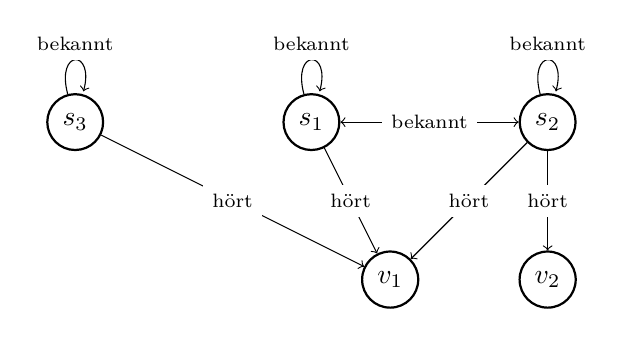
\begin{tikzpicture}
        \begin{scope}[every node/.style={circle,draw,thick}]
            \node (s1) at (0, 2) {$s_1$};
            \node (s2) at (3, 2) {$s_2$};
            \node (s3) at (-3, 2) {$s_3$};
            \node (v1) at (1, 0) {$v_1$};
            \node (v2) at (3, 0) {$v_2$};
        \end{scope}
        \begin{scope}[every node/.style={fill=white}]
            \path [->] (s1) edge node {\scriptsize{hört}} (v1);
            \path [->] (s2) edge node {\scriptsize{hört}} (v1);
            \path [->] (s3) edge node {\scriptsize{hört}} (v1);
            \path [->] (s2) edge node {\scriptsize{hört}} (v2);
            \path [<->] (s1) edge node {\scriptsize{bekannt}} (s2);
            \path [->] (s1) edge [loop above] node {\scriptsize{bekannt}} (s1);
            \path [->] (s2) edge [loop above] node {\scriptsize{bekannt}} (s2);
            \path [->] (s3) edge [loop above] node {\scriptsize{bekannt}} (s3);
        \end{scope}
    \end{tikzpicture}
    \end{center}
    \begin{align*}
        (\text{VL} \sqcap \text{PflichtVL})^\MI &= \{v_1, v_2\} \cap \{v_1\} = \{v_1\}\\
        \neg\text{VL}^\MI &= \{s_1, s_2, s_3\}\\
        (\text{Student} \sqcup \text{VL})^\MI &= \Delta^\MI\\
        (\exists \text{bekanntMit}.\text{Student})^\MI &= \{s_1, s_2, s_3\}\\
        (\exists \text{bekanntMit}.\exists\text{bekanntMit}.\text{Student})^\MI &= \{s_1, s_2, s_3\}\\
        (\forall \text{hört}.\text{PflichtVL})^\MI &= \{s_1, s_3, v_1, v_2\}
    \end{align*}
\end{tafel}

Verwendete Symbole:

\begin{itemize}
  \item $\MI$, $\MJ$ für Interpretationen
  \item $d$, $e$ für Elemente der Domäne
\end{itemize}

Für Interpretationen verwenden wir übliche Terminologie für Graphen:

\begin{itemize}
  \item $e$ für $r$-Nachfolger von $d$ (in $\MI$) wenn ($d$, $e$) $\in r^\MI$
  \item $e$ für $r$-Vorgänger von $d$ (in $\MI$) wenn ($e$, $d$) $\in r^\MI$
  \item wenn $r$ unwichtig, sprechen wir nun von Nachfolgern / Vorgängern
  \item $\MI$ ist endlich gdw. $\Delta^\MI$ endlich ist.
\end{itemize}

\subsubsection{Extension/Modell}
\label{sec:exetension}

Wir nennen
\begin{itemize}
\item
  $C^\MI$ ist \emph{Extension} des Konzeptes oder der Rolle $C$
\item
    jedes $d \in C^\MI$ ist eine \emph{Instanz} des Konzeptes $C$
\item $r^\MI$ die \emph{Extension} der Rolle r.
\end{itemize}

Beachte, das $\top^\MI$ für jede Interpretation $\MI$ identisch mit
$\Delta^\MI$ ist. Intuitiv entspricht $\top$ der Menge alle Elemente.
$\bot^\MI$ ist für jede Interpretation $\MI$ leer, repräsentiert also
intuitiv, dass etwas unmöglich ist, z.B.:
\begin{align*}
    &\text{Mensch} \sqcap \forall \text{hatKind}.\bot\\
    &\text{Menschen, die keine Kinder haben}
\end{align*}

\begin{tafel}[Beweis $\top^\MI = \Delta^\MI$]
    \begin{align*}
        \top^\MI &= (A \sqcup \neq A)^\MI = A^\MI \cup (\neg A)^\MI\\
                 &= A^\MI \cup (\Delta^\MI \setminus A^\MI)\\
                 &= \Delta^\MI
    \end{align*}
\end{tafel}

\subsubsection{Erfüllbarkeit, Subsumtion, Äquivalenz}
\label{sec:erfull-subsum-equiv}
\label{erfuxfcllbarkeit-subsumtion-uxe4quivalenz}

\begin{definition}[Erfüllbar, subsumiert, äquivalent]
    \mbox{}\\Seien $C$ und $D$ $\ALC$-Konzepte. Dann
\begin{itemize}
\item
  ist $C$ \emph{erfüllbar}, wenn es eine Interpretation $\MI$ gibt mit
  $C^\MI \neq \emptyset$. $\MI$ ist dann ein \emph{Modell} von
  $C$.
\item
  wird $C$ von $D$ \emph{subsumiert}, wenn $C^\MI \subseteq D^\MI$
  in allen Interpretationen $\MI$ (Notation $C \sqsubseteq D$)
\item
  sind C und D \emph{äquivalent}, wenn $C^\MI = D^\MI$ in allen
  Interpretationen $\MI$ (Notation $C \equiv D$)
\end{itemize}
\end{definition}

\begin{tafel} [Beispiel Nichterfüllbarkeit und Subsumtion]\mbox{}
    \begin{enumerate}[label=\alph*)]
        \item $C = \exists r.A \sqcap \forall r.\neg A$ ist nicht erfüllbar.
            \begin{proof}
                Angenommen es gibt eine Interpretation $\MI$ mit $C^\MI \neq \emptyset$. Sei $d\in C^\MI$, wegen $d \in (\exists r.A)^\MI$ gibt es $e \in A^\MI$ mit $(d, e) \in r^\MI$. Wegen $d \in (\forall r.\neg A)^\MI$ gilt $e\in \neg A^\MI$. Folglich kann es kein Element $d \in C^\MI$ geben.
            \end{proof}
        \item $\exists r.(A\sqcap B) \sqsubseteq  \exists r.A \sqcap \exists r.B$
            \begin{proof}
                Sei $\MI$ Interpretation und $d \in (\exists r. (A\sqcap B))^\MI$. Dann gibt es $e \in (A\sqcap B)^\MI$ mit $(d, e) \in r^\MI$, wegen $e \in A^\MI$ gilt $d \in (\exists r.A)^\MI$ und wegen $e \in B^\MI$ gilt $d \in (\exists r.B)^\MI$. Folglich gilt auch $d \in (\exists r.A \sqcap \exists r.B)^\MI$.
            \end{proof}
    \end{enumerate}
\end{tafel}

Es gelten die üblichen aussagenlogischen Äquivalenzen, wie z.B. das de
Morgansche Gesetz.

\subsection{TBoxen}\label{tboxen}
\label{sec:tbox}

TBoxen(\enquote{terminologische Boxen}) definieren Konzepte und setzen diese zueinander in Beziehung.

\begin{definition}[TBox-Syntax]
\emph{Konzeptinklusion} ist Ausdruck $C \sqsubseteq D$ mit $C$, $D$ Konzepten.
Eine \emph{TBox} ist eine endliche Menge von Konzeptinklusionen.  Wir
verwenden $C \equiv D$ als Abkürzung für $C \sqsubseteq D$, $D \sqsubseteq C$.
\end{definition}
Wir lesen $C \sqsubseteq D$ als \enquote{$C$ impliziert $D$}.

\begin{definition}[TBox, Semantik] 
Eine Interpretation $\MI$
\begin{itemize}
\item
  erfüllt Konzeptinklusion $C \sqsubseteq D$ gdw.
  $C^\MI \subseteq D^\MI$
\item
  ist Modell von TBox $\MT$ gdw. $\MI$ alle Konzeptinklusionen in $\MT$
  erfüllt
\end{itemize}
\end{definition}

\begin{tafel}[Beispiel Model von $\MT$]
    \label{t25}
    \begin{align*}
        \MT = \{& \text{Student} \equiv \text{Mensch} \sqcap \exists \text{hört}.\text{VL},\\
                &\text{VL} \equiv \text{PflichtVL} \sqcup \text{WahlVL},\\
                &\text{Student} \sqcap \exists \text{hört}.\text{VL} \sqsubseteq \exists \text{bekanntMit}.\text{Student},\\
                &\text{PflichtVL} \sqcap \text{WahlVL} \sqsubseteq \bot\}
    \end{align*}
    Model $\MI$ von $\MT$:
    \begin{center}
    \begin{tikzpicture}
        \begin{scope}[every node/.style={circle,thick,draw}]
            \node (s3) at (0, -2) {};
            \node (s1) at (0, 0) {};
            \node (s2) at (3, 0) {};
        \end{scope}
        \begin{scope}[every node/.style={fill=white}]
            \path [->] (s1) edge node {\scriptsize{hört}} (s3);
            \path [->] (s1) edge node {\scriptsize{bekannt}} (s2);
            \path [->] (s1) edge [loop left] node {\scriptsize{bekannt}} (s1);
            \node (l1) at (s1) [above = 1mm of s1] {\small{Mensch}};
            \node at (l1) [above = 0mm of l1] {\small{Student}};
            \node at (s2) [above = 1mm of s2] {\small{Mensch}};
            \node (l2) at (s3) [left = 1mm of s3] {\small{VL}};
            \node at (l2) [below = 0mm of l2] {\small{PflichtVL}};
        \end{scope}
    \end{tikzpicture}
    \end{center}
    $\MI$ erfüllt auch $\text{Student} \sqsubseteq \exists \text{bekanntMit}.\text{Mensch}$ und $\text{VL} \equiv \text{PlfichtVL}$.
\end{tafel}

Intuitiv entsprechen Interpretationen mögliche Welten, TBoxen hingegen schließen Welten aus, die wir für nicht möglich halten. Jede Konzeptinklusion \enquote{eliminiert} un\-erwünsch\-te Interpretationen.

\subsubsection{Modellierung}\label{modellierung}

In der Praxis bestehen TBoxen zu einem großen Teil aus:

\begin{itemize}
\item Konzeptinklusion $A \sqsubseteq C$, wobei $A$ ein Konzeptname ist: $C$ ist notwendige Bedingung dafür, eine Instanz von $A$ zu sein
\item Konzeptdefinition $A \equiv C$, wobei $A$ ein Konzeptname ist: $C$ ist notwendige und hinreichende Bedingung dafür, eine Instanz von $A$ zu sein.
    Hinreichende Bedingungen sind für viele Konzepte schwer zu finden.
    \end{itemize}
Modellierungsmuster, die nicht in dieses Schema passen sind z.B.:
\begin{itemize}
\item Disjunktheitsconstraints $C \sqcap D \sqsubseteq \bot$: Kein Objekt kann gleichzeitig zu $C$ und $D$ gehören
\item Komplexe Zusammenhänge zwischen mehreren Konzepten. Zum Beispiel:
    \begin{align*}
        \mathit{Professor} \sqcap \exists \mathit{hat}.\mathit{Lehrdeputat} \sqsubseteq \exists \mathit{haelt}.\mathit{Vorlesung}
    \end{align*}
\end{itemize}

\subsubsection{Erfüllbarkeit, Subsumtion, Äquivalenz}
\label{sec:tbox-erfuellbarkeit}
\label{erfuxfcllbarkeit-subsumtion-uxe4quivalenz-1}

\begin{definition}[Erfüllbar, subsumiert, äquivalent bezüglich einer TBox] 
Seien $C$, $D$, $\ALC$-Konzepte und $\MT$ TBox. Dann

\begin{itemize}
  \item ist $C$ \emph{erfüllbar bzgl.} $\MT$ gdw. $\MT$ Modell $\MI$ hat mit $C^\MI \neq \emptyset$
  \item wird $C$ \emph{von} $D$ \emph{subsumiert bzgl.} $\MT$, wenn $C^\MI \subseteq D^\MI$ in allen Modellen $\MI$ von $\MT$ (Notation $\MT \models C \sqsubseteq D$)
  \item sind $C$ und $D$ \emph{äquivalent bzgl.} $\MT$, gdw. $C^\MI = D^\MI$ in allen Modellen $\MI$ von $\MT$ (Notation $\MT \models C \equiv D$)
\end{itemize}
\end{definition}

Intuitiv gesprochen ist diese Definition wie in
\autoref{sec:erfull-subsum-equiv}, nur ist $\MI$ jeweils Modell von einer TBox
$\MT$.

\begin{tafel}[Beispiel Erfüllbarkeit, Subsumtion, Äquivalenz bezüglich $\MT$]\mbox{}
    \begin{enumerate}[label=\alph*)]
    \item Sei $\MT$ die TBox aus \autoref{t25} und $C = \text{Student} \sqcap \forall \text{hört}.\text{PflichtVL}$. $C$ ist erfüllbar bezüglich $\MT$, denn folgende Interpretation $\MI$ ist Modell von $\MT$ mit $C^\MI$
    \begin{center}
    \begin{tikzpicture}
        \begin{scope}[every node/.style={circle,thick,draw}]
            \node (s3) at (0, -2) {};
            \node (s1) at (0, 0) {};
        \end{scope}
        \begin{scope}[every node/.style={fill=white}]
            \path [->] (s1) edge node {\scriptsize{hört}} (s3);
            \path [->] (s1) edge [loop right] node {\scriptsize{bekannt}} (s1);
            \node at (s1) [left = 1mm of s1] {\small{Mensch}};
            \node at (s1) [below left = 1mm of s1] {\small{Student}};
            \node at (s3) [left = 1mm of s3] {\small{VL}};
            \node at (s3) [below left = 1mm of s3] {\small{PflichtVL}};
        \end{scope}
    \end{tikzpicture}
    \end{center}
\item Sei $\MT$ wieder aus \autoref{t25} und $C = \text{Student} \sqcap \exists \text{hört}.\text{PflichtVL} \sqcap \forall \text{hört}.\text{WahlVL}$.
    $C$ ist unerfüllbar bezüglich $\MT$: Nimm im Gegenteil an $C$ sei erfüllbar bezüglich $\MT$, dann gibt es Modell $\MI$ und Instanz $d\in C^\MI$. Nach Semantik von $\sqcap$ gilt $d \in (\exists \text{hört}.\text{PflichtVL})^\MI$. Also gibt es ein $e \in (\text{PflichtVL})^\MI$ mit $(d, e) \in \text{hört}^\MI$. Wegen $d \in (\forall \text{hört}.\text{WahlVL})^\MI$ gilt $e \in \text{WahlVL}^\MI$. Also ist $e \in (\text{PflichtVL} \sqcap \text{WahlVL})^\MI$, was $(\text{PflichtVL} \sqcap \text{WahlVL}) \in \bot$ verletzt. Folglich kann es keine Interpretation geben.
\item Sei $\MT$ wie oben und $C = \text{Student}, D = \exists \text{bekanntMit}.\text{Student}$. Es gilt $\MT \models C \sqsubseteq D$. Sei $\MI$ Modell von $\MT$ und $d \in \text{Student}^\MI$. Zu zeigen $d \in (\exists \text{bekanntMit}.\text{Student})^\MI$. Wegen Zeile 1 von $\MT$ gilt $d \in (\exists \text{hört}.\text{VL})^\MI$, also ist $d \in (\text{Student} \sqcap \exists \text{hört}.\text{VL})^\MI$. Aus Zeile 3 von $\MT$ folgt wie gewünscht $d \in (\exists \text{bekanntMit}.\text{Student})^\MI$.
    \end{enumerate}
\end{tafel}

Hinweise für Beweisstrategien:
\begin{itemize}
\item Erfüllbarkeit zeigen: Modell angeben
\item Unerfüllbarkeit zeigen: semantisch argumentieren
\item Subsumtion zeigen: semantisch Argumentieren
\item Nicht-Subsumtion zeigen: Gegenmodell angeben
\end{itemize}

\subsubsection{Monotonie}\label{monotonie}
Das Erweitern einer TBox um zusätzliche Konzeptinklusionen wirkt sich wie folgt auf Erfüllbarkeit und Subsumtion aus:

\begin{lemma}[TBox Monotonie]
\label{lem:tbox-monoton}
Seien $\MT_1$ und $\MT_2$ TBoxen mit $\MT_1 \subseteq \MT_2$. Dann gilt:
\begin{enumerate}
\item
  Wenn $C$ erfüllbar bzgl. $\MT_2$, dann ist $C$ erfüllbar bzgl.
  $\MT_1$.
\item
  Wenn $\MT_1 \models C \sqsubseteq D$, dann
  $\MT_2 \models C \sqsubseteq D$.
\end{enumerate}
\end{lemma}

\begin{tafel}[Beweisskizze von TBox Monotonie]Beweisskizze von \autoref{lem:tbox-monoton}
\begin{enumerate}
  \item \begin{proof}
      Sei $C$ erfüllbar bzgl. $\MT_2$.
  Dann gibt es Modell $\MI$ von $\MT_2$ mit $C^\MI \neq \emptyset$.
  Also erfüllt $\MI$ alle Konzeptinklusionen in $\MT_2$ und wegen $\MT_1 \subseteq \MT_2$ auch alle Konzeptinklusionen in $\MT_1$.
  Also ist $\MI$ Modell von $\MT_1$ mit $C^\MI \neq \emptyset$.
  Also ist $C$ erfüllbar bzgl. $\MT_1$.
  \end{proof}
  \item \begin{proof}
    Kontraposition: Wenn $\MT_2 \not\models C \sqsubseteq D$ dann $\MT_1 \not\models C \sqsubseteq D$. \\
  Es gelte $\MT_2 \not\models C \sqsubseteq D$.
  D.h. es gibt Modell $\MI$ von $\MT_2$ mit $C^\MI \not\subseteq D^\MI$.
  Wie im 1. Falls ist $\MI$ auch Modell von $\MT_1 \subseteq \MT_2$.
  Also $\MT_1 \not\models C \sqsubseteq D$
  \end{proof}
\end{enumerate}

Die umgekehrten Aussagen sind im Allgemeinen nicht richtig. Beispiel:
\begin{align*}
    &\MT_1 = \emptyset, \MT_2 = \{A \sqsubseteq B\}\\
    &\MT_1 \subseteq \MT_2 \\
    &\MT_2 \models A \sqsubseteq B\\
    &\MT_1 \models A \sqsubseteq B
\end{align*}
\end{tafel}

Eine Logik, die diese Eigenschaften erfüllt, nennt man \emph{monoton} (das Hinzunehmen von Formeln kann nur zu \emph{zusätzlichen} Konsequenzen, führen, aber nicht dazu, dass Konsequenzen ungültig werden)

\subsection{Schlussfolgerungsprobleme}\label{schlussfolgerungsprobleme}

Schlussfolgern dient dazu aus explizit gegebenes Wissen neues Wissen abzuleiten, das vorher nur implizit vorhanden war. Beschreibungslogiken sind so designed, dass sie so viel Ausdrucksstärke wie nötig, aber nicht mehr, besitzen, um möglichst effizientes Schlussfolgern zu Erlauben.

Die von uns betrachteten Schlussfolgerungsprobleme sind:

\begin{itemize}
  \item \textbf{Erfüllbarkeitsproblem}: Gegeben $C$ und $\MT$, entscheide ob $C$ erfüllbar bzgl. $\MT$.
  \item \textbf{Subsumtionsproblem}: Gegeben $C$, $D$ und $\MT$, entscheide ob $\MT \models C \sqsubseteq D$
  \item \textbf{Äquivalenzproblem}: Gegeben $C$, $D$ und $\MT$, entscheide ob $\MT \models C \equiv D$
\end{itemize}

Diese Entscheidungsprobleme können auch mit leerer TBox $\MT = \emptyset$ betrachtet werden.

Die Schlussfolgerungsprobleme werden dazu genutzt Modellierungsfehler in Ontologien zu finden, die Struktur der TBox explizit zu machen und um Redundanzen zu finden.

\subsubsection{Subsumtion als Ordnungsrelation}\label{subordn}

\begin{lemma}[TBox Subsumtion ist fast partielle Ordnung]
    Für jede TBox $\MT$ ist die Relation \enquote{$\sqsubseteq$ bzgl. $\MT$}

\begin{itemize}
  \item reflexiv ($\MT \models C \sqsubseteq C$) und
  \item transitiv ($\MT \models C \sqsubseteq D$ und $\MT \models D \sqsubseteq E$ impliziert $\MT \models C \sqsubseteq E$).
\end{itemize}
Bis auf die fehlende Antisymmetrie ($xRy \wedge yRx \rightarrow x = y$) ist $\sqsubseteq$ also eine partielle Ordnung.
\end{lemma}

Man kann $\sqsubseteq$ als Hasse-Diagram darstellen, dessen Knoten mit Mengen von Konzepten beschriftet sind.

\begin{tafel}[Beispiel Hasse-Diagram]\mbox{}
    \begin{align*}
        \MT = \{&\text{Mensch} \equiv \text{Mann} \sqcup \text{Frau}, \text{Mensch} \sqsubseteq \text{Säugetier}\\
               &\text{Frau} \sqsubseteq \neg\text{Mann}\\
               &\text{NMM} \equiv \text{Mensch} \sqcap \neg\text{Mann}\}
    \end{align*}
    \begin{center}
    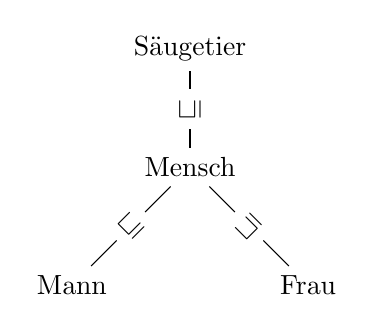
\begin{tikzpicture}
        \begin{scope}[every node/.style={fill=white}]
            \node (s1) at (0, 0) {Mann};
            \node (s2) at (3, 0) {Frau};
            \node (s3) at (1.5, 1.5) {Mensch};
            \node (s4) at (1.5, 3) {Säugetier};
        \end{scope}
        \begin{scope}[every node/.style={fill=white}]
            \path [-] (s1) edge node [rotate=45] {$\sqsubseteq$} (s3);
            \path [-] (s2) edge node [rotate=135] {$\sqsubseteq$} (s3);
            \path [-] (s3) edge node [rotate=90] {$\sqsubseteq$} (s4);
        \end{scope}
    \end{tikzpicture}
\end{center}
\end{tafel}

\subsubsection{Klassifikation}

Ein weiteres Schlussforlgerungsproblem:

\begin{itemize}
  \item \textbf{Klassifikation}: Gegeben $\MT$, berechne das Hasse Diagramm für $\sqsubseteq$ bzgl. $\MT$, eingeschränkt auf Konzeptnamen in $\MT$.
\end{itemize}

Dies ist ein Berechnungsproblem (kein Entscheidungsproblem), das in der Praxis durch $n^2$ Subsumtionsberchnungen berechenbar ist und für das zahlreiche Optimierungen verfügbar sind ($n$ = Anzahl der Konzeptnamen in $\MT$).

\subsubsection{Reduktion}

Die Schlussfolgerungsprobleme sind wechselseitig polynomiell aufeinander reduzierbar:

\begin{lemma}[Schlussfolgerungsprobleme sind wechselseitig reduzierbar]\mbox{}
\begin{enumerate}
\item{\emph{Erfüllbarkeit} auf \emph{Nicht-Äquivalenz} \\
$C$ erfüllbar bzgl. $\MT$ gdw. $\MT \not\models C \equiv \bot$}
\item{\emph{Subsumtion} auf \emph{Unerfüllbarkeit} \\
$\MT \models C \sqsubseteq D$ gdw. $C \sqcap \neg D$ unerfüllbar bzgl.
$\MT$
\item{\emph{Äquivalenz} auf \emph{Subsumtion} \\}
$\MT \models C \equiv D$ gdw. $\MT \models \top \sqsubseteq \left( C \sqcap D \right) \sqcup \left( \neg C \sqcap \neg D \right)$}
\end{enumerate}
\end{lemma}

Dies heißt für uns, dass ein Algorithmus für eines der Probleme auch für die
anderen beiden verwendet werden kann. Alle drei Probleme haben dieselbe
Komplexität (in $\ALC$). Daher werden wir uns im Folgenden hauptsächlich auf
Erfüllbarkeit konzentrieren.

\begin{tafel}[Exemplarische Reduktion von Schlussfolgerungsproblemen]\mbox{}
    \begin{center} \begin{tabular}{ll}
        $T \models C \sqsubseteq D$ & gdw. für alle Modelle $\MI$ von $\MT$ $C^\MI \subseteq D^\MI$\\
                                    & gdw. es gibt kein Modell $\MI$ von $\MT$ bei dem $C^\MI \not\subseteq D^\MI$\\
                                    & gdw. es gibt kein Modell $\MI$ von $\MT$ bei dem $(C \sqcap \neg D)^\MI \neq \emptyset$\\
                                    & gdw. $C \sqcap \neg D$ unerfüllbar bezüglich $\MT$\\
    \end{tabular}
\end{center}
\end{tafel}

\subsection{Erweiterungen von \texorpdfstring{$\ALC$}{ALC}}\label{erweiterungen-von-alc}

Wir betrachten exemplarisch die beiden Erweiterungen $\ALCI$ und $\ALCQ$ von $\ALC$. Es existieren viel mehr Erweiterungen (z.B.: um spezielle Rolleniterpretationen, temporale Operatoren etc.). Diese können auch kombiniert werden, z.B.: $\ALCQI$.

\subsubsection{Inverse Rollen (\texorpdfstring{$\ALCI$}{ALCI})}\label{inverse-rollen-alci}

Zunächst betrachten wir $\ALCI$, das $\ALC$ um die Möglichkeit inverse Rollen in Existenz- und Werterestriktionen zu benutzen erweitert.

\begin{definition}[Inverse Rollen]
Für jeden Rollennamen $r$ ist $r^{-}$ die \emph{inverse
Rolle} zu $r$. Wir definieren
$\left( r^{-} \right)^\MI = \left\{ \left( e,d \right)\  \right|\ \left( d,e \right) \in r^\MI\}$
\end{definition}

\begin{tafel}[Beispiel Nützlichkeit von Inversen]
    \begin{align*}
        \MT = \{& \text{Professor} \sqsubseteq \text{Verrückt} \sqcap \exists  \text{gibt}.\text{Vorlesung}\\
                & \text{Vorlesung} \sqsubseteq \forall \text{wirdGegebenVon}.\neg\text{Verrückt}\}
    \end{align*}
    Das folgende ist ein Modell von $\MT$, da es keine wirdGegebenVon-Kante gibt und man die intuitive Bedeutung der Kante in $\ALC$ nicht erzwingen kann.
    \begin{center}
    \begin{tikzpicture}
        \begin{scope}[every node/.style={circle,thick,draw}]
            \node (s1) at (0, 0) {};
            \node (s2) at (2, 0) {};
        \end{scope}
        \begin{scope}[every node/.style={fill=white}]
            \path [->] (s1) edge node {\scriptsize{gibt}} (s2);
            \node at (s1) [left = 1mm of s1] {\small{Professor}};
            \node at (s1) [below left = 1mm of s1] {\small{Verrückt}};
            \node at (s2) [right = 1mm of s2] {\small{Vorlesung}};
        \end{scope}
    \end{tikzpicture}
    \end{center}
    Mit der Verwendung von Inversen lässt sich Zeile 2 von $\MT$ neu definieren, wodurch das Modell $\MT$ nicht mehr erfüllt.
    \begin{align*}
        \text{Vorlesung} \sqsubseteq \forall \text{gibt}^-.\neg\text{Verrückt}
    \end{align*}
\end{tafel}

\subsubsection{Zahlenrestriktion (\texorpdfstring{$\ALCQ$}{ALCQ})}\label{zahlenrestriktion-alcq}

\begin{definition}[Zahlenrestriktion]
Für jede natürliche Zahl $n$, jeden Rollennamen $r$ und
jedes Konzept $C$:

\begin{itemize}
  \item $\left( \leq n\ r\ C \right)$ (Höchstens-Restriktion)
  \item $\left( \geq n\ r\ C \right)$ (Mindestens-Restriktion)
\end{itemize}

Die Semantik ist \begin{align*}
    \left( \leq n\ r\ C \right)^\MI &= \left\{ d \in \Delta^\MI\ |\ \#\left\{ e\ |\ \left( d,e \right) \in r^\MI \land e \in C^\MI \right\} \leq n \right\}\\
    ( \geq n\ r\ C)^\MI &= \left\{ d \in \Delta^\MI\ |\ \#\left\{ e\ |\ \left( d,e \right) \in r^\MI \land e \in C^\MI \right\} \geq n \right\}
\end{align*}
\end{definition}

\begin{tafel}[TODO]
    %TODO
\end{tafel}

Beachte:

\begin{itemize}
  \item $\exists r.C$ ist äquivalent zu $(\geq 1\ r\ C)$
  \item $\forall r.C$ ist äquivalent zu $(\leq 0\ r\ \neg C)$
\end{itemize}

\subsection*{Literatur für dieses Kapitel}

Basis:

\fullcite{handbook}
